
%%%%%%%%%%%%%%%%%%%%%%%%%%%%%%%%%%%%%%%%%%%%%%%%%%%%%%%%%%%%%%%%%%%%%%%%%%%%%%
% Copyright (c) 2003-2014 by University of Queensland
% http://www.uq.edu.au
%
% Primary Business: Queensland, Australia
% Licensed under the Open Software License version 3.0
% http://www.opensource.org/licenses/osl-3.0.php
%
% Development until 2012 by Earth Systems Science Computational Center (ESSCC)
% Development 2012-2013 by School of Earth Sciences
% Development from 2014 by Centre for Geoscience Computing (GeoComp)
%
%%%%%%%%%%%%%%%%%%%%%%%%%%%%%%%%%%%%%%%%%%%%%%%%%%%%%%%%%%%%%%%%%%%%%%%%%%%%%%

\chapter{The \escript Module}\label{ESCRIPT CHAP}

\section{Concepts}
\escript is a \PYTHON module that allows you to represent the values of
a function at points in a \Domain in such a way that the function will
be useful for the Finite Element Method (FEM) simulation. It also
provides what we call a function space that describes how the data is
used in the simulation. Stored along with the data is information
about the elements and nodes which will be used by the domain (e.g. \finley).

\subsection{Function spaces}
In order to understand what we mean by the term 'function space',
consider that the solution of a partial differential
equation\index{partial differential equation} (PDE) is a function on a domain
$\Omega$.  When solving a PDE using FEM, the solution is
piecewise-differentiable but, in general, its gradient is discontinuous.
To reflect these different degrees of smoothness, different function spaces
are used.
For instance, in FEM, the displacement field is represented by its values at
the nodes of the mesh, and so is continuous.
The strain, which is the symmetric part of the gradient of the displacement
field, is stored on the element centers, and so is considered to be
discontinuous.

A function space is described by a \FunctionSpace object.
The following statement generates the object \var{solution_space} which is
a \FunctionSpace object and provides access to the function space of
PDE solutions on the \Domain \var{mydomain}:

\begin{python}
  solution_space=Solution(mydomain)
\end{python}
The following generators for function spaces on a \Domain \var{mydomain} are commonly used:
\begin{itemize}
\item \var{Solution(mydomain)}: solutions of a PDE
\item \var{ReducedSolution(mydomain)}: solutions of a PDE with a reduced
    smoothness requirement, e.g. using a lower order approximation on the same
    element or using macro elements\index{macro elements}
\item \var{ContinuousFunction(mydomain)}: continuous functions, e.g. a temperature distribution
\item \var{Function(mydomain)}: general functions which are not necessarily continuous, e.g. a stress field
\item \var{FunctionOnBoundary(mydomain)}: functions on the boundary of the domain, e.g. a surface pressure
\item \var{FunctionOnContact0(mydomain)}: functions on side $0$ of a discontinuity
\item \var{FunctionOnContact1(mydomain)}: functions on side $1$ of a discontinuity
\end{itemize}
In some cases under-integration is used. For these cases the user may use a
\FunctionSpace from the following list:
\begin{itemize}
\item \var{ReducedFunction(mydomain)}
\item \var{ReducedFunctionOnBoundary(mydomain)}
\item \var{ReducedFunctionOnContact0(mydomain)}
\item \var{ReducedFunctionOnContact1(mydomain)}
\end{itemize}
In comparison to the corresponding full version they use a reduced number of
integration nodes (typically one only) to represent values.

\begin{figure}
\centering
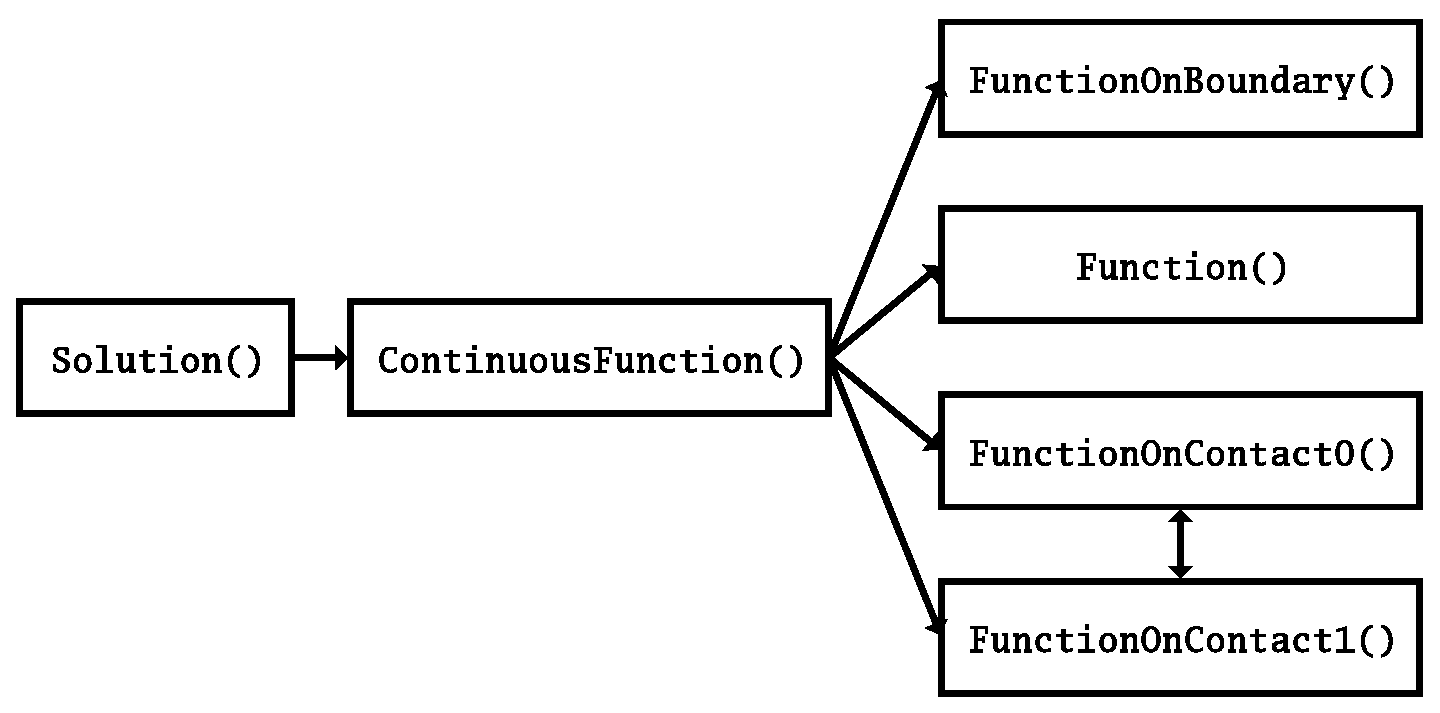
\includegraphics{EscriptDiagram1}
\caption{\label{ESCRIPT DEP}Dependency of function spaces in \finley.
An arrow indicates that a function in the \FunctionSpace at the starting point
can be interpolated to the \FunctionSpace of the arrow target.
All function spaces above the dotted line can be interpolated to any of
the function spaces below the line. See also \Sec{SEC Projection}.}
\end{figure}

The reduced smoothness for a PDE solution is often used to fulfill the
Ladyzhenskaya-Babuska-Brezzi condition~\cite{LBB} when solving saddle point
problems\index{saddle point problems}, e.g. the Stokes equation.
A discontinuity\index{discontinuity} is a region within the domain across
which functions may be discontinuous.
The location of a discontinuity is defined in the \Domain object.
\fig{ESCRIPT DEP} shows the dependency between the types of function spaces
in \finley (other libraries may have different relationships).

The solution of a PDE is a continuous function. Any continuous function can
be seen as a general function on the domain and can be restricted to the
boundary as well as to one side of a discontinuity (the result will be
different depending on which side is chosen). Functions on any side of the
discontinuity can be seen as a function on the corresponding other side.

A function on the boundary or on one side of the discontinuity cannot be seen
as a general function on the domain as there are no values defined for the
interior. For most PDE solver libraries the space of the solution and
continuous functions is identical, however in some cases, for example when
periodic boundary conditions are used in \finley, a solution fulfills periodic
boundary conditions while a continuous function does not have to be periodic.

The concept of function spaces describes the properties of functions and
allows abstraction from the actual representation of the function in the
context of a particular application. For instance, in the FEM context a
function of the \Function type (written as \emph{Function()} in \fig{ESCRIPT DEP})
is usually represented by its values at the element center,
but in a finite difference scheme the edge midpoint of cells is preferred.
By changing its function space you can use the same function in a Finite
Difference scheme instead of Finite Element scheme.
Changing the function space of a particular function will typically lead to
a change of its representation.
So, when seen as a general function, a continuous function which is typically
represented by its values on the nodes of the FEM mesh or finite difference
grid must be interpolated to the element centers or the cell edges,
respectively. Interpolation happens automatically in \escript whenever it is
required\index{interpolation}. The user needs to be aware that an
interpolation is not always possible, see \fig{ESCRIPT DEP} for \finley.
An alternative approach to change the representation (=\FunctionSpace) is
projection\index{projection}, see \Sec{SEC Projection}.

\subsection{\Data Objects}
In \escript the class that stores these functions is called \Data.
The function is represented through its values on \DataSamplePoints where
the \DataSamplePoints are chosen according to the function space of the
function.
\Data class objects are used to define the coefficients of the PDEs to be
solved by a PDE solver library and also to store the solutions of the PDE.

The values of the function have a rank which gives the number of indices,
and a \Shape defining the range of each index.
The rank in \escript is limited to the range 0 through 4 and it is assumed
that the rank and \Shape is the same for all \DataSamplePoints.
The \Shape of a \Data object is a tuple (list) \var{s} of integers.
The length of \var{s} is the rank of the \Data object and the \var{i}-th
index ranges between 0 and $\var{s[i]}-1$.
For instance, a stress field has rank 2 and \Shape $(d,d)$ where $d$ is the
number of spatial dimensions.
The following statement creates the \Data object \var{mydat} representing a
continuous function with values of \Shape $(2,3)$ and rank $2$:
\begin{python}
  mydat=Data(value=1, what=ContinuousFunction(myDomain), shape=(2,3))
\end{python}
The initial value is the constant 1 for all \DataSamplePoints and all
components.

\Data objects can also be created from any \numpy array or any object, such
as a list of floating point numbers, that can be converted into
a \numpyNDA\cite{NUMPY}.
The following two statements create objects which are equivalent
to \var{mydat}:
\begin{python}
  mydat1=Data(value=numpy.ones((2,3)), what=ContinuousFunction(myDomain))
  mydat2=Data(value=[[1,1], [1,1], [1,1]], what=ContinuousFunction(myDomain))
\end{python}
In the first case the initial value is \var{numpy.ones((2,3))} which generates
a $2 \times 3$ matrix as an instance of \numpyNDA filled with ones.
The \Shape of the created \Data object is taken from the \Shape of the array.
In the second case, the creator converts the initial value, which is a list of
lists, into a \numpyNDA before creating the actual \Data object.

For convenience \escript provides creators for the most common types
of \Data objects in the following forms (\var{d} defines the spatial
dimensionality):
\begin{itemize}
\item \code{Scalar(0, Function(mydomain))} is the same as \code{Data(0, Function(myDomain),(,))}\\
    (each value is a scalar), e.g. a temperature field
\item \code{Vector(0, Function(mydomain))} is the same as \code{Data(0, Function(myDomain),(d,))}\\
    (each value is a vector), e.g. a velocity field
\item \code{Tensor(0, Function(mydomain))} equals \code{Data(0, Function(myDomain), (d,d))},
    e.g. a stress field
\item \code{Tensor4(0,Function(mydomain))} equals \code{Data(0,Function(myDomain), (d,d,d,d))},
    e.g. a Hook tensor field
\end{itemize}
Here the initial value is 0 but any object that can be converted into
a \numpyNDA and whose \Shape is consistent with \Shape of the \Data object to
be created can be used as the initial value.

\Data objects can be manipulated by applying unary operations (e.g. cos, sin,
log), and they can be combined point-wise by applying arithmetic operations
(e.g. +, - ,* , /).
We emphasize that \escript itself does not handle any spatial dependencies as
it does not know how values are interpreted by the processing PDE solver library.
However \escript invokes interpolation if this is needed during data manipulations.
Typically, this occurs in binary operations when the arguments belong to
different function spaces or when data are handed over to a PDE solver library
which requires functions to be represented in a particular way.

The following example shows the usage of \Data objects. Assume we have a
displacement field $u$ and we want to calculate the corresponding stress field
$\sigma$ using the linear-elastic isotropic material model
\begin{eqnarray}\label{eq: linear elastic stress}
\sigma_{ij}=\lambda u_{k,k} \delta_{ij} + \mu ( u_{i,j} + u_{j,i})
\end{eqnarray}
where $\delta_{ij}$ is the Kronecker symbol and
$\lambda$ and $\mu$ are the Lam\'e coefficients. The following function
takes the displacement \var{u} and the Lam\'e coefficients \var{lam} and \var{mu}
as arguments and returns the corresponding stress:
\begin{python}
  from esys.escript import *
  def getStress(u, lam, mu):
    d=u.getDomain().getDim()
    g=grad(u)
    stress=lam*trace(g)*kronecker(d)+mu*(g+transpose(g))
    return stress
\end{python}
The variable \var{d} gives the spatial dimensionality of the domain on which
the displacements are defined.
\var{kronecker} returns the Kronecker symbol with indices $i$ and $j$ running
from 0 to \var{d}-1.
The call \var{grad(u)} requires the displacement field \var{u} to be in
the \var{Solution} or \ContinuousFunction.
The result \var{g} as well as the returned stress will be in the \Function.
If, for example, \var{u} is the solution of a PDE then \code{getStress} might
be called in the following way:
\begin{python}
  s=getStress(u, 1., 2.)
\end{python}
However \code{getStress} can also be called with \Data objects as values for
\var{lam} and \var{mu} which, for instance in the case of a temperature
dependency, are calculated by an expression.
The following call is equivalent to the previous example:
\begin{python}
  lam=Scalar(1., ContinuousFunction(mydomain))
  mu=Scalar(2., Function(mydomain))
  s=getStress(u, lam, mu)
\end{python}
%
The function \var{lam} belongs to the \ContinuousFunction but with \var{g} the
function \var{trace(g)} is in the \Function.
In the evaluation of the product \var{lam*trace(g)} we have different function
spaces (on the nodes versus in the centers) and at first glance we have incompatible data.
\escript converts the arguments into an appropriate function space according
to \fig{ESCRIPT DEP}.
In this example that means \escript sees \var{lam} as a function of the \Function.
In the context of FEM this means the nodal values of \var{lam} are
interpolated to the element centers.
The interpolation is automatic and requires no special handling.

\begin{figure}
\centering
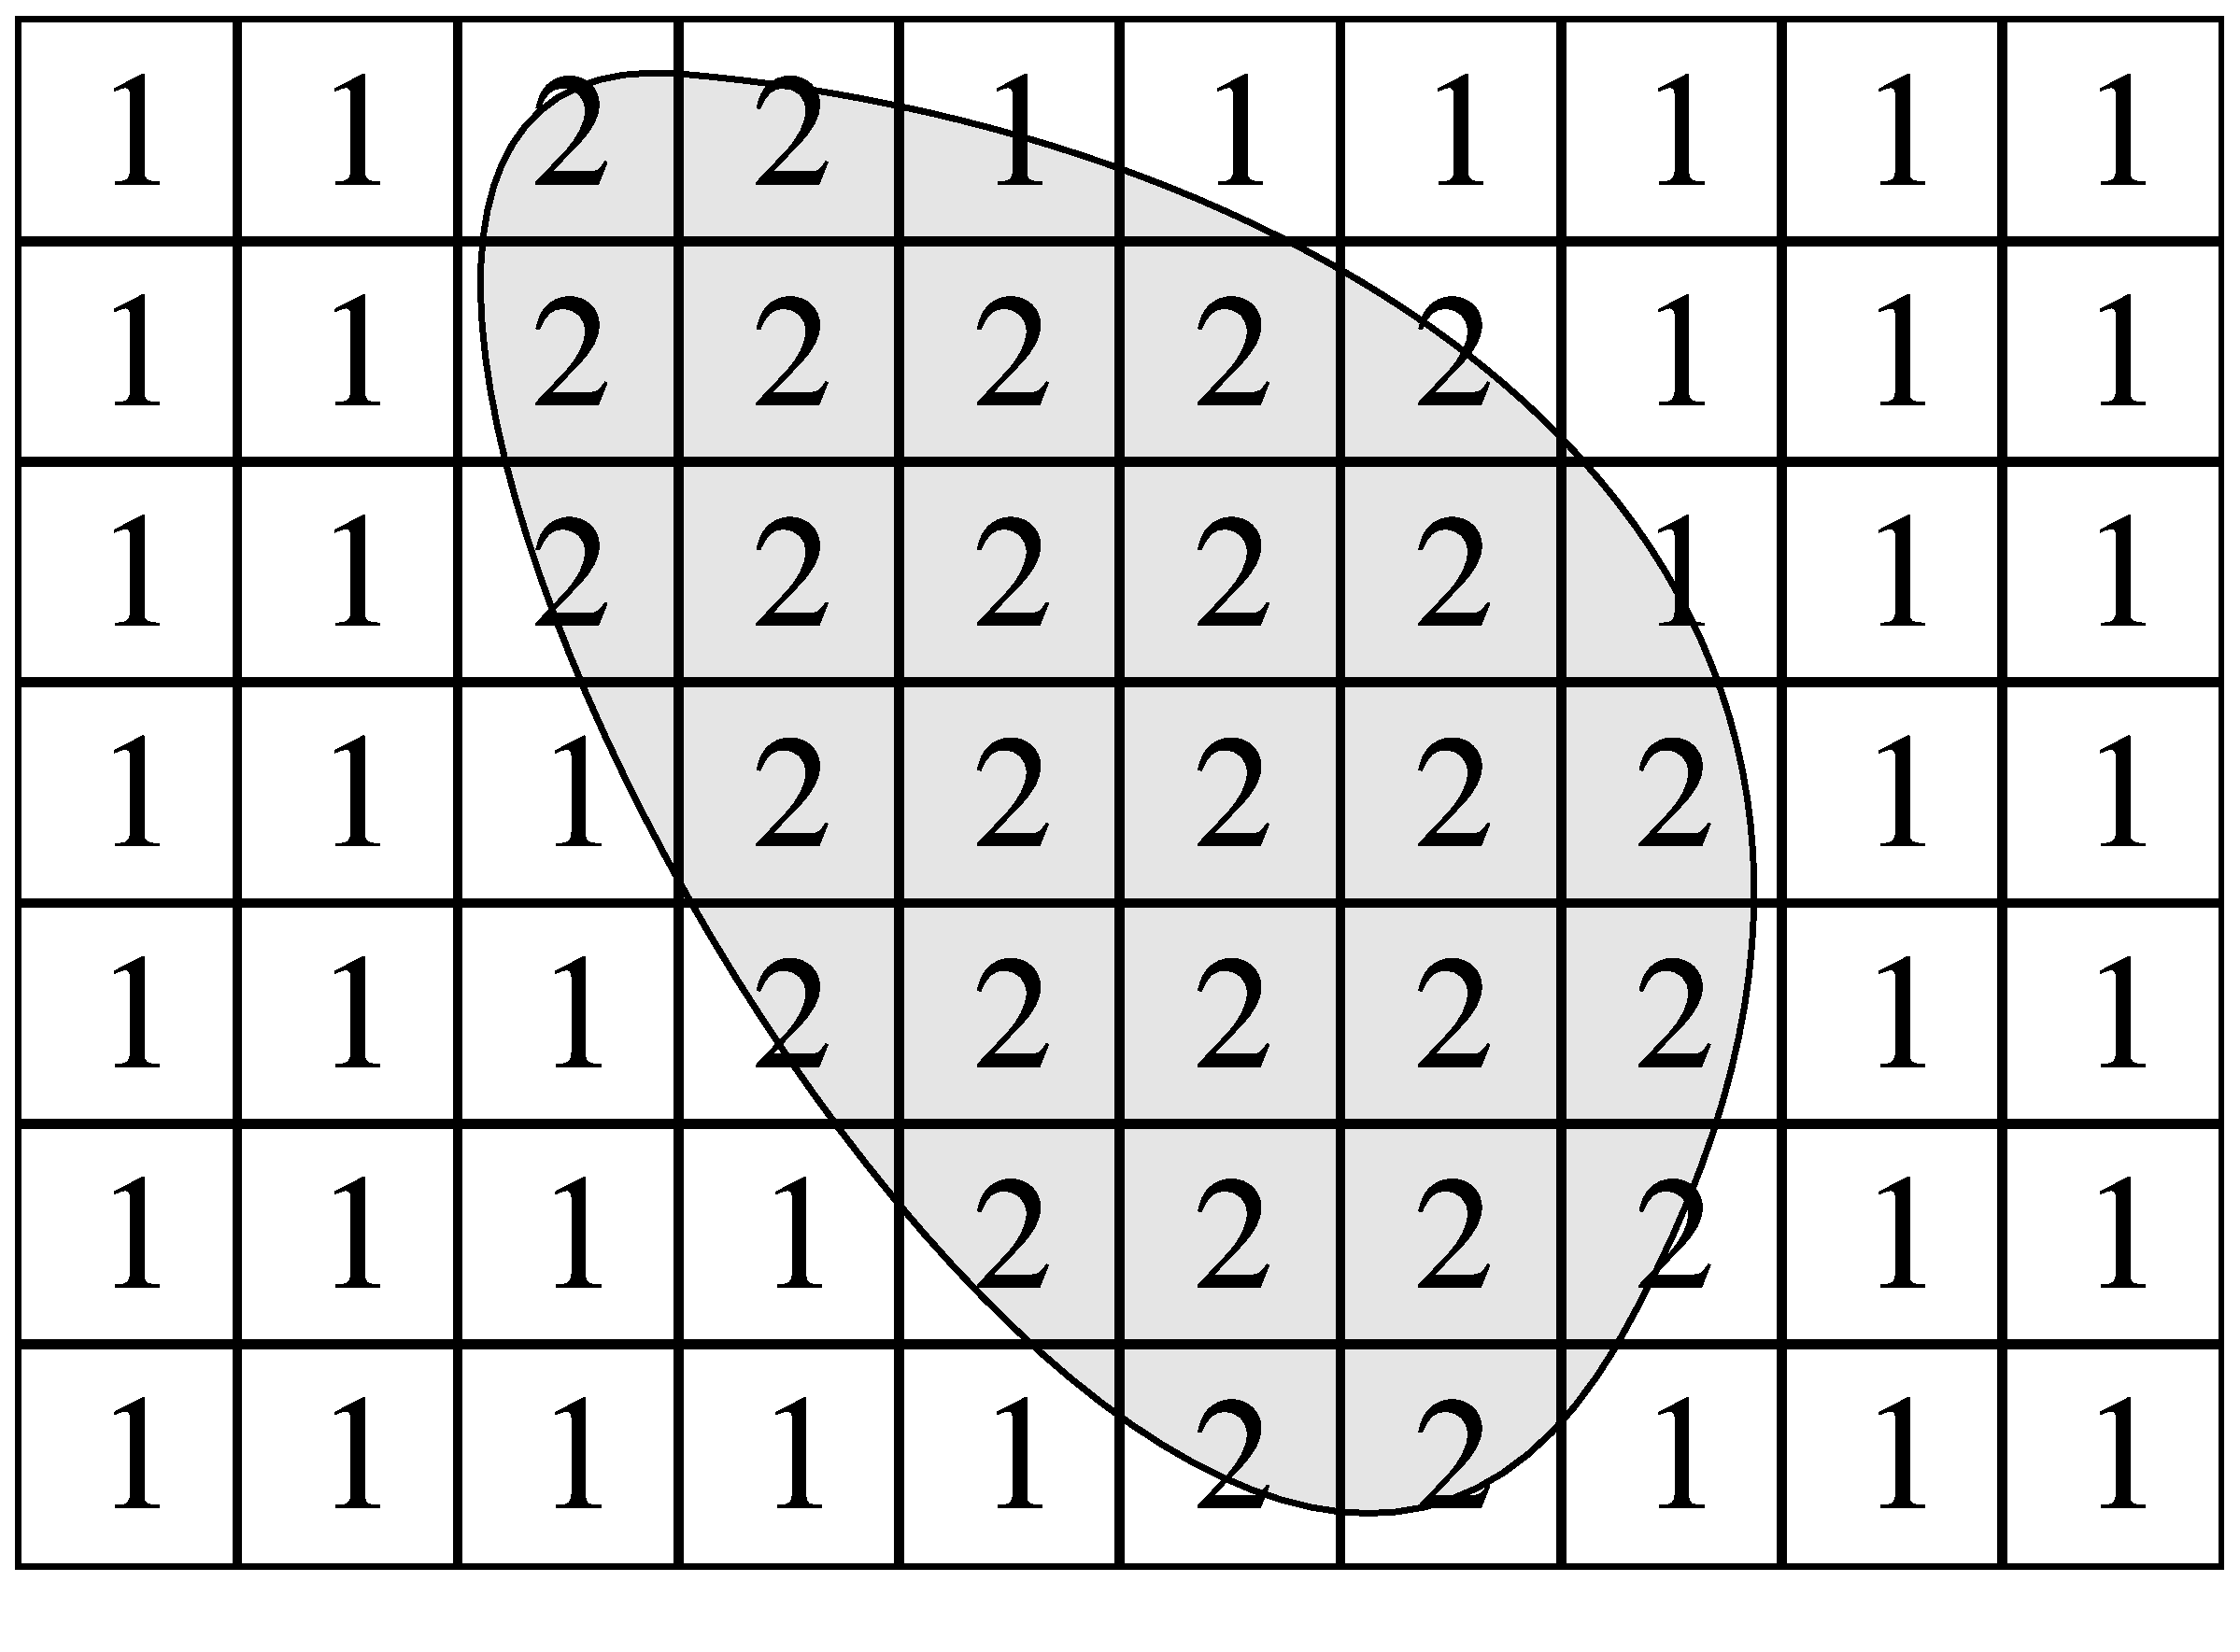
\includegraphics{EscriptDiagram2}
\caption{\label{Figure: tag}Element Tagging. A rectangular mesh over a region
with two rock types {\it white} and {\it gray} is shown.
The number in each cell refers to the major rock type present in the cell
($1$ for {\it white} and $2$ for {\it gray}).}
\end{figure}

\subsection{Tagged, Expanded and Constant Data}
Material parameters such as the Lam\'e coefficients are typically dependent on
rock types present in the area of interest.
A common technique to handle these kinds of material parameters is
\emph{tagging}\index{tagging}, which uses storage efficiently.
\fig{Figure: tag} shows an example. In this case two rock types {\it white}
and {\it gray} can be found in the domain.
The domain is subdivided into triangular shaped cells.
Each cell has a tag indicating the rock type predominantly found in this cell.
Here $1$ is used to indicate rock type {\it white} and $2$ for rock type {\it gray}.
The tags are assigned at the time when the cells are generated and stored in
the \Domain class object. To allow easier usage of tags, names can be used
instead of numbers. These names are typically defined at the time when the
geometry is generated.

The following statements show how to use tagged values for \var{lam} as shown
in \fig{Figure: tag} for the stress calculation discussed above:
\begin{python}
  lam=Scalar(value=2., what=Function(mydomain))
  insertTaggedValue(lam, white=30., gray=5000.)
  s=getStress(u, lam, 2.)
\end{python}
In this example \var{lam} is set to $30$ for those cells with tag {\it white}
(=$1$) and to $5000$ for cells with tag {\it gray} (=$2$).
The initial value $2$ of \var{lam} is used as a default value for the case
when a tag is encountered which has not been linked with a value.
The \code{getStress} method does not need to be changed now that we are using tags.
\escript resolves the tags when \var{lam*trace(g)} is calculated.

This brings us to a very important point about \escript.
You can develop a simulation with constant Lam\'e coefficients, and then later
switch to tagged Lam\'e coefficients without otherwise changing your \PYTHON script.
In short, you can use the same script for models with different domains and
different types of input data.

There are three main ways in which \Data objects are represented internally --
constant, tagged, and expanded.
In the constant case, the same value is used at each sample point while only a
single value is stored to save memory.
In the expanded case, each sample point has an individual value (such as for the solution of a PDE).
This is where your largest data sets will be created because the values are
stored as a complete array.
The tagged case has already been discussed above.
Expanded data is created when specifying \code{expanded=True} in the \Data
object constructor, while tagged data requires calling the \member{insertTaggedValue}
method as shown above.

Values are accessed through a sample reference number.
Operations on expanded \Data objects have to be performed for each sample
point individually.
When tagged values are used, the values are held in a dictionary.
Operations on tagged data require processing the set of tagged values only,
rather than processing the value for each individual sample point.
\escript allows any mixture of constant, tagged and expanded data in a single expression.

\subsection{Saving and Restoring Simulation Data}
\Data objects can be written to disk files with the \member{dump} method and
read back using the \member{load} method, both of which use the
\netCDF\cite{NETCDF} file format.
Use these to save data for checkpoint/restart or simply to save and reuse data
that was expensive to compute.
For instance, to save the coordinates of the data points of a
\ContinuousFunction to the file \file{x.nc} use
\begin{python}
  x=ContinuousFunction(mydomain).getX()
  x.dump("x.nc")
  mydomain.dump("dom.nc")
\end{python}
To recover the object \var{x}, and you know that \var{mydomain} was an \finley
mesh, use
\begin{python}
  from esys.finley import LoadMesh
  mydomain=LoadMesh("dom.nc")
  x=load("x.nc", mydomain)
\end{python}
Obviously, it is possible to execute the same steps that were originally used
to generate \var{mydomain} to recreate it. However, in most cases using
\member{dump} and \member{load} is faster, particularly if optimization has
been applied.
If \escript is running on more than one \MPI process \member{dump} will create
an individual file for each process containing the local data.
In order to avoid conflicts the \MPI processor
rank is appended to the file names.
That is instead of one file \file{dom.nc} you would get
\file{dom.nc.0000}, \file{dom.nc.0001}, etc.
You still call \code{LoadMesh("dom.nc")} to load the domain but you have to
make sure that the appropriate file is accessible from the corresponding rank,
and loading will only succeed if you run with as many processes as were used
when calling \member{dump}.

The function space of the \Data is stored in \file{x.nc}.
If the \Data object is expanded, the number of data points in the file and of
the \Domain for the particular \FunctionSpace must match.
Moreover, the ordering of the values is checked using the reference
identifiers provided by the \FunctionSpace on the \Domain.
In some cases, data points will be reordered so be aware and confirm that you
get what you wanted.

A more flexible way of saving and restoring \escript simulation data
is through an instance of the \class{DataManager} class.
It has the advantage of allowing to save and load not only a \Domain and
\Data objects but also other values\footnote{The \PYTHON \emph{pickle} module
is used for other types.} you compute in your simulation script.
Further, \class{DataManager} objects can simultaneously create files for
visualization so no extra calls to \code{saveVTK} etc. are needed.

The following example shows how the \class{DataManager} class can be used.
For an explanation of all member functions and options see the class reference
Section \ref{sec:datamanager}.
\begin{python}
  from esys.escript import DataManager, Scalar, Function
  from esys.finley import Rectangle

  dm = DataManager(formats=[DataManager.RESTART, DataManager.VTK])
  if dm.hasData():
    mydomain=dm.getDomain()
    val=dm.getValue("val")
    t=dm.getValue("t")
    t_max=dm.getValue("t_max")
  else:
    mydomain=Rectangle()
    val=Function(mydomain).getX()
    t=0.
    t_max=2.5

  while t<t_max:
    t+=.01
    val=val+t/2
    dm.addData(val=val, t=t, t_max=t_max)
    dm.export()
\end{python}
In the constructor we specify that we want \code{RESTART} (i.e. dump) files
and \code{VTK} files to be saved.
By default, the constructor will look for previously saved \code{RESTART}
files under the current directory and load them.
We can then enquire if such files were found by calling the \member{hasData}
method. If it returns \True we retrieve the domain and values into local
variables. Otherwise the same variables are initialized with appropriate
values to start a new simulation.
Note, that \var{t} and \var{t_max} are regular floating point values and not
\Data objects. Yet they are treated the same way by the \class{DataManager}.

After this initialization step the script enters the main simulation loop
where calculations are performed.
When these are finalized for a time step we call the \member{addData} method
to let the manager know which variables to store on disk.
This does not actually save the data yet and it is allowed to call
\member{addData} more than once to add information incrementally, e.g. from
separate functions that have access to the \class{DataManager} instance.
Once all variables have been added the \member{export} method has to be called
to flush all data to disk and clear the manager.
In this example, this call dumps \var{mydomain} and \var{val} to files
in a restart directory and also stores \var{t} and \var{t_max} on disk.
Additionally, it generates a \VTK file for visualization of the data.
If the script would stop running before its completion for some reason (e.g.
because its runtime limit was exceeded in a batch job environment), you could
simply run it again and it would resume at the point it stopped before.

\section{\escript Classes}

\subsection{The \Domain class}
\begin{classdesc}{Domain}{}
A \Domain object is used to describe a geometric region together with
a way of representing functions over this region.
The \Domain class provides an abstract interface to the domain of \FunctionSpace and \Data objects.
\Domain needs to be subclassed in order to provide a complete implementation.
\end{classdesc}

\vspace{1em}\noindent The following methods are available:
\begin{methoddesc}[Domain]{getDim}{}
    returns the number of spatial dimensions of the \Domain.
\end{methoddesc}
%
\begin{methoddesc}[Domain]{dump}{filename}
    writes the \Domain to the file \var{filename} using the \netCDF file format.
\end{methoddesc}
%
\begin{methoddesc}[Domain]{getX}{}
    returns the locations in the \Domain. The \FunctionSpace of the returned
    \Data object is chosen by the \Domain implementation. Typically it will be
    in the \ContinuousFunction.
\end{methoddesc}
%
\begin{methoddesc}[Domain]{setX}{newX}
    assigns new locations to the \Domain. \var{newX} has to have \Shape $(d,)$
    where $d$ is the spatial dimensionality of the domain. Typically \var{newX}
    must be in the \ContinuousFunction but the space actually to be used
    depends on the \Domain implementation. Not all domain families support
    setting locations.
\end{methoddesc}
%
\begin{methoddesc}[Domain]{getNormal}{}
    returns the surface normals on the boundary of the \Domain as a \Data object.
\end{methoddesc}
%
\begin{methoddesc}[Domain]{getSize}{}
    returns the local sample size, i.e. the element diameter, as a \Data object.
\end{methoddesc}
%
\begin{methoddesc}[Domain]{setTagMap}{tag_name, tag}
    defines a mapping of the tag name \var{tag_name} to the \var{tag}.
\end{methoddesc}
%
\begin{methoddesc}[Domain]{getTag}{tag_name}
    returns the tag associated with the tag name \var{tag_name}.
\end{methoddesc}
%
\begin{methoddesc}[Domain]{isValidTagName}{tag_name}
    returns \True if \var{tag_name} is a valid tag name.
\end{methoddesc}
%
\begin{methoddesc}[Domain]{__eq__}{arg}
    (\PYTHON \var{==} operator) returns \True if the \Domain \var{arg}
    describes the same domain, \False otherwise.
\end{methoddesc}
%
\begin{methoddesc}[Domain]{__ne__}{arg}
    (\PYTHON \var{!=} operator) returns \True if the \Domain \var{arg} does
    not describe the same domain, \False otherwise.
\end{methoddesc}
%
\begin{methoddesc}[Domain]{__str__}{}
    (\PYTHON \var{str()} function) returns a string representation of the
    \Domain.
\end{methoddesc}
%
\begin{methoddesc}[Domain]{onMasterProcessor}{}
    returns \True if the process is the master process within the \MPI
    process group used by the \Domain. This is the process with rank 0.
    If \MPI support is not enabled the return value is always \True.
\end{methoddesc}
%
\begin{methoddesc}[Domain]{getMPISize}{}
    returns the number of \MPI processes used for this \Domain. If \MPI
    support is not enabled 1 is returned.
\end{methoddesc}
%
\begin{methoddesc}[Domain]{getMPIRank}{}
    returns the rank of the process executing the statement within the
    \MPI process group used by the \Domain. If \MPI support is not enabled
    0 is returned.
\end{methoddesc}
%
\begin{methoddesc}[Domain]{MPIBarrier}{}
    executes barrier synchronization within the \MPI process group used by
    the \Domain. If \MPI support is not enabled, this command does nothing.
\end{methoddesc}

\subsection{The \FunctionSpace class}
\begin{classdesc}{FunctionSpace}{}
\FunctionSpace objects, which are instantiated by generator functions, are
used to define properties of \Data objects such as continuity.
A \Data object in a particular \FunctionSpace is represented by its values at
\DataSamplePoints which are defined by the type and the \Domain of the \FunctionSpace.
\end{classdesc}

\vspace{1em}\noindent The following methods are available:
%
\begin{methoddesc}[FunctionSpace]{getDim}{}
    returns the spatial dimensionality of the \Domain of the \FunctionSpace.
\end{methoddesc}
%
\begin{methoddesc}[FunctionSpace]{getX}{}
    returns the location of the \DataSamplePoints.
\end{methoddesc}
%
\begin{methoddesc}[FunctionSpace]{getNormal}{}
    If the domain of functions in the \FunctionSpace is a hyper-manifold (e.g.
    the boundary of a domain) the method returns the outer normal at each of
    the \DataSamplePoints. Otherwise an exception is raised.
\end{methoddesc}
%
\begin{methoddesc}[FunctionSpace]{getSize}{}
    returns a \Data object measuring the spacing of the \DataSamplePoints.
    The size may be zero.
\end{methoddesc}
%
\begin{methoddesc}[FunctionSpace]{getDomain}{}
    returns the \Domain of the \FunctionSpace.
\end{methoddesc}
%
\begin{methoddesc}[FunctionSpace]{setTags}{new_tag, mask}
    assigns a new tag \var{new_tag} to all data samples where \var{mask} is
    positive for a least one data point.
    \var{mask} must be defined on this \FunctionSpace.
    Use the \var{setTagMap} to assign a tag name to \var{new_tag}.
\end{methoddesc}
%
\begin{methoddesc}[FunctionSpace]{__eq__}{arg}
    (\PYTHON \var{==} operator) returns \True if the \FunctionSpace \var{arg}
    describes the same function space, \False otherwise.
\end{methoddesc}
%
\begin{methoddesc}[FunctionSpace]{__ne__}{arg}
    (\PYTHON \var{!=} operator) returns \True if the \FunctionSpace \var{arg}
    does not describe the same function space, \False otherwise.
\end{methoddesc}

\begin{methoddesc}[Domain]{__str__}{}
    (\PYTHON \var{str()} function) returns a string representation of the
    \FunctionSpace.
\end{methoddesc}

\noindent The following functions provide generators for \FunctionSpace objects:

\begin{funcdesc}{Function}{domain}
    returns the \Function on the \Domain \var{domain}. \Data objects in this
    type of \Function are defined over the whole geometric region defined by
    \var{domain}.
\end{funcdesc}
%
\begin{funcdesc}{ContinuousFunction}{domain}
    returns the \ContinuousFunction on the \Domain domain. \Data objects in
    this type of \Function are defined over the whole geometric region defined
    by \var{domain} and assumed to represent a continuous function.
\end{funcdesc}
%
\begin{funcdesc}{FunctionOnBoundary}{domain}
    returns the \FunctionOnBoundary on the \Domain domain. \Data objects in
    this type of \Function are defined on the boundary of the geometric region
    defined by \var{domain}.
\end{funcdesc}
%
\begin{funcdesc}{FunctionOnContactZero}{domain}
    returns the \FunctionOnContactZero the \Domain domain. \Data objects in
    this type of \Function are defined on side 0 of a discontinuity  within
    the geometric region defined by \var{domain}.
    The discontinuity is defined when \var{domain} is instantiated.
\end{funcdesc}
%
\begin{funcdesc}{FunctionOnContactOne}{domain}
    returns the \FunctionOnContactOne on the \Domain domain. \Data objects in
    this type of \Function are defined on side 1 of a discontinuity within
    the geometric region defined by \var{domain}.
    The discontinuity is defined when \var{domain} is instantiated.
\end{funcdesc}
%
\begin{funcdesc}{Solution}{domain}
    returns the \SolutionFS on the \Domain domain. \Data objects in this type
    of \Function are defined on the geometric region defined by \var{domain}
    and are solutions of partial differential equations\index{partial differential equation}.
\end{funcdesc}
%
\begin{funcdesc}{ReducedSolution}{domain}
    returns the \ReducedSolutionFS on the \Domain domain. \Data objects in
    this type of \Function are defined on the geometric region defined by
    \var{domain} and are solutions of partial differential
    equations\index{partial differential equation} with a reduced smoothness
    for the solution approximation.
\end{funcdesc}

\subsection{The \Data Class}
\label{SEC ESCRIPT DATA}

The following table shows arithmetic operations that can be performed
point-wise on \Data objects:
\begin{center}
    \begin{tabular}{l|l}
        \textbf{Expression} & \textbf{Description}\\
        \hline
        \code{+arg} & identical to \var{arg}\index{+}\\
        \code{-arg} & negation of \var{arg}\index{-}\\
        \code{arg0+arg1} & adds \var{arg0} and \var{arg1}\index{+}\\
        \code{arg0*arg1} & multiplies \var{arg0} and \var{arg1}\index{*}\\
        \code{arg0-arg1} & subtracts \var{arg1} from \var{arg0}\index{-}\\
        \code{arg0/arg1} & divides \var{arg0} by \var{arg1}\index{/}\\
        \code{arg0**arg1} & raises \var{arg0} to the power of \var{arg1}\index{**}\\
    \end{tabular}
\end{center}
At least one of the arguments \var{arg0} or \var{arg1} must be a \Data object.
Either of the arguments may be a \Data object, a \PYTHON number or a \numpy
object.
If \var{arg0} or \var{arg1} are not defined on the same \FunctionSpace, then
an attempt is made to convert \var{arg0} to the \FunctionSpace of \var{arg1}
or to convert \var{arg1} to the \FunctionSpace of \var{arg0}.
Both arguments must have the same \Shape or one of the arguments may be of
rank 0 (a constant).
The returned \Data object has the same \Shape and is defined on
the \DataSamplePoints as \var{arg0} or \var{arg1}.

The following table shows the update operations that can be applied to
\Data objects:
\begin{center}
    \begin{tabular}{l|l}
        \textbf{Expression} & \textbf{Description}\\
        \hline
        \code{arg0+=arg1} & adds \var{arg1} to \var{arg0}\index{+}\\
        \code{arg0*=arg1} & multiplies \var{arg0} by \var{arg1}\index{*}\\
        \code{arg0-=arg1} & subtracts \var{arg1} from\var{arg0}\index{-}\\
        \code{arg0/=arg1} & divides \var{arg0} by \var{arg1}\index{/}\\
        \code{arg0**=arg1} & raises \var{arg0} to the power of \var{arg1}\index{**}\\
    \end{tabular}
\end{center}
\var{arg0} must be a \Data object. \var{arg1} must be a \Data object or an
object that can be converted into a \Data object.
\var{arg1} must have the same \Shape as \var{arg0} or have rank 0.
In the latter case it is assumed that the values of \var{arg1} are constant
for all components. \var{arg1} must be defined in the same \FunctionSpace as
\var{arg0} or it must be possible to interpolate \var{arg1} onto the
\FunctionSpace of \var{arg0}.

The \Data class supports taking slices as well as assigning new values to a
slice of an existing \Data object\index{slicing}.
The following expressions for taking and setting slices are valid:
\begin{center}
    \begin{tabular}{l|ll}
        \textbf{Rank of \var{arg}} & \textbf{Slicing expression} & \textbf{\Shape of returned and assigned object}\\
        \hline
        0 & no slicing & N/A\\
        1 & \var{arg[l0:u0]} & (\var{u0}-\var{l0},)\\
        2 & \var{arg[l0:u0,l1:u1]} & (\var{u0}-\var{l0},\var{u1}-\var{l1})\\
        3 & \var{arg[l0:u0,l1:u1,l2:u2]} & (\var{u0}-\var{l0},\var{u1}-\var{l1},\var{u2}-\var{l2})\\
        4 & \var{arg[l0:u0,l1:u1,l2:u2,l3:u3]} & (\var{u0}-\var{l0},\var{u1}-\var{l1},\var{u2}-\var{l2},\var{u3}-\var{l3})\\
    \end{tabular}
\end{center}
Let \var{s} be the \Shape of \var{arg}, then
\begin{align*}
0 \le \var{l0} \le \var{u0} \le \var{s[0]},\\
0 \le \var{l1} \le \var{u1} \le \var{s[1]},\\
0 \le \var{l2} \le \var{u2} \le \var{s[2]},\\
0 \le \var{l3} \le \var{u3} \le \var{s[3]}.
\end{align*}
Any of the lower indexes \var{l0}, \var{l1}, \var{l2} and \var{l3} may not be
present in which case $0$ is assumed.
Any of the upper indexes \var{u0}, \var{u1}, \var{u2} and \var{u3} may be
omitted, in which case the upper limit for that dimension is assumed.
The lower and upper index may be identical in which case the column and the
lower or upper index may be dropped.
In the returned or in the object assigned to a slice, the corresponding
component is dropped, i.e. the rank is reduced by one in comparison to \var{arg}.
The following examples show slicing in action:
\begin{python}
  t=Data(1., (4,4,6,6), Function(mydomain))
  t[1,1,1,0]=9.
  s=t[:2,:,2:6,5] # s has rank 3
  s[:,:,1]=1.
  t[:2,:2,5,5]=s[2:4,1,:2]
\end{python}


\subsection{Generation of \Data objects}
\begin{classdesc}{Data}{value=0, shape=(,), what=FunctionSpace(), expanded=\False}
creates a \Data object with \Shape \var{shape} in the \FunctionSpace \var{what}.
The values at all \DataSamplePoints are set to the double value \var{value}.
If \var{expanded} is \True the \Data object is represented in expanded form.
\end{classdesc}

\begin{classdesc}{Data}{value, what=FunctionSpace(), expanded=\False}
creates a \Data object in the \FunctionSpace \var{what}.
The value for each data sample point is set to \var{value}, which could be a
\numpy object, \Data object or a dictionary of \numpy or floating point
numbers. In the latter case the keys must be integers and are used as tags.
The \Shape of the returned object is equal to the \Shape of \var{value}.
If \var{expanded} is \True the \Data object is represented in expanded form.
\end{classdesc}

\begin{classdesc}{Data}{}
creates an \EmptyData object. The \EmptyData object is used to indicate that
an argument is not present where a \Data object is required.
\end{classdesc}

\begin{funcdesc}{Scalar}{value=0., what=FunctionSpace(), expanded=\False}
returns a \Data object of rank 0 (a constant) in the \FunctionSpace \var{what}.
Values are initialized with \var{value}, a double precision quantity.
If \var{expanded} is \True the \Data object is represented in expanded form.
\end{funcdesc}

\begin{funcdesc}{Vector}{value=0., what=FunctionSpace(), expanded=\False}
returns a \Data object of \Shape \var{(d,)} in the \FunctionSpace \var{what},
where \var{d} is the spatial dimension of the \Domain of \var{what}.
Values are initialized with \var{value}, a double precision quantity.
If \var{expanded} is \True the \Data object is represented in expanded form.
\end{funcdesc}

\begin{funcdesc}{Tensor}{value=0., what=FunctionSpace(), expanded=\False}
returns a \Data object of \Shape \var{(d,d)} in the \FunctionSpace \var{what},
where \var{d} is the spatial dimension of the \Domain of \var{what}.
Values are initialized with \var{value}, a double precision quantity.
If \var{expanded} is \True the \Data object is represented in expanded form.
\end{funcdesc}

\begin{funcdesc}{Tensor3}{value=0., what=FunctionSpace(), expanded=\False}
returns a \Data object of \Shape \var{(d,d,d)} in the \FunctionSpace \var{what},
where \var{d} is the spatial dimension of the \Domain of \var{what}.
Values are initialized with \var{value}, a double precision quantity.
If \var{expanded} is \True the \Data object is represented in expanded form.
\end{funcdesc}

\begin{funcdesc}{Tensor4}{value=0., what=FunctionSpace(), expanded=\False}
returns a \Data object of \Shape \var{(d,d,d,d)} in the \FunctionSpace \var{what},
where \var{d} is the spatial dimension of the \Domain of \var{what}.
Values are initialized with \var{value}, a double precision quantity.
If \var{expanded} is \True the \Data object is represented in expanded form.
\end{funcdesc}

\begin{funcdesc}{load}{filename, domain}
recovers a \Data object on \Domain \var{domain} from the file \var{filename},
which was created by \function{dump}.
\end{funcdesc}

\subsection{Generating random \Data objects}
A \Data object filled with random values can be produced using the
\function{RandomData} function.
By default values are drawn uniformly at random from the interval $[0,1]$ (i.e.
including end points).
The function takes a shape for the data points and a \FunctionSpace for the new
\Data as arguments.
For example:
\begin{python}
from esys.finley import *
from esys.escript import *

domain=Rectangle(11,11)
fs=ContinuousFunction(domain)
d=RandomData((), fs)
\end{python}
would result in \var{d} being filled with scalar random data since \texttt{()}
is an empty tuple.

\begin{python}
from esys.finley import *
from esys.escript import *

domain=Rectangle(11,11)
fs=ContinuousFunction(domain)
d=RandomData((2,2), fs)
\end{python}
would give \var{d} the same number of data points, but each point would be a
$2\times 2$ matrix instead of a scalar.

By default, the seed used to generate the random values will be different each
time.
If required, you can specify a seed to ensure the same sequence is produced.
\begin{python}
from esys.dudley import *
from esys.escript import *

seed=-17171717
domain=Brick(10,10,10)
fs=Function(domain)
d=RandomData((2,2), fs, seed)
\end{python}

The \var{seed} can be any integer value\footnote{which can be converted to a
C++ long} but 0 is special.
A seed of zero will cause \escript to use a different seed each time.
Also, note that the mechanism used to produce the random values could be
different in different releases.

\noindent\textbf{Note for MPI users:}
\textsl{
Even if you specify a seed, you will only get the same results if you are running with the same
number of ranks.
If you change the number of ranks, you will get different values for the same seed.
}

\subsubsection{Smoothed randoms}
The \ripley domains (see Chapter \ref{chap:ripley}) support generating random
scalars which are smoothed using Gaussian blur.
To use this, you need to supply the radius of the filter kernel (in elements)
and the \var{sigma} value used in the filter.
For example:
\begin{python}
from esys.ripley import *
from esys.escript import *

fs=ContinuousFunction(Rectangle(11,11, d1=2,d0=2))
d=RandomData((), fs, 0, ('gaussian', 1, 0.5))
\end{python}
will use a filter that uses the immediate neighbours of each point with a sigma
value of $0.5$.
The random values will be different each time this code is executed due to the
seed of $0$.

Ripley's Gaussian smoothing has the following requirements:
\begin{enumerate}
    \item If \MPI is in use, then each rank must have at least $5$ elements in
          it \emph{in each dimension}. This value increases as the radius of
          the blur increases.
    \item The data being generated must be scalar. (You can generate random
          data objects for \ripley domains with whatever shape you require, you
          just can't smooth them unless that shape is scalar).
\end{enumerate}
An exception will be raised if either of these requirements is not met. 

The components of the matrix used in the kernal for the 2D case are
defined\cite{gaussfilter} by:

\[ G(x,y) = \frac{1}{2\pi\sigma^2} e^{-\frac{x^2+y^2}{2\sigma^2}} \]

\noindent For the 3D case, we use:

\[ G(x,y) = \frac{1}{(\sqrt{2\pi\sigma^2})^3} e^{-\frac{x^2+y^2+z^2}{2\sigma^2}} \]

All distances ($x$,$y$,$z$) refer to the number of points from the centre point. 
That is, the closest neighbours have at least one distance of $1$, the next
``ring'' of neighbours have at least one $2$ and so on.
The matrix is normalised before use.

\subsection{\Data methods}
These are the most frequently used methods of the \Data class.
A complete list of methods can be found in the reference guide,
see \ReferenceGuide.

\begin{methoddesc}[Data]{getFunctionSpace}{}
returns the \FunctionSpace of the object.
\end{methoddesc}

\begin{methoddesc}[Data]{getDomain}{}
returns the \Domain of the object.
\end{methoddesc}

\begin{methoddesc}[Data]{getShape}{}
returns the \Shape of the object as a \class{tuple} of integers.
\end{methoddesc}

\begin{methoddesc}[Data]{getRank}{}
returns the rank of the data on each data point\index{rank}.
\end{methoddesc}

\begin{methoddesc}[Data]{isEmpty}{}
returns \True if the \Data object is the \EmptyData object, \False otherwise.
Note that this is not the same as asking if the object contains no \DataSamplePoints.
\end{methoddesc}

\begin{methoddesc}[Data]{setTaggedValue}{tag_name, value}
assigns the \var{value} to all \DataSamplePoints which have the tag
assigned to \var{tag_name}. \var{value} must be an object of class
\class{numpy.ndarray} or must be convertible into a \class{numpy.ndarray} object.
\var{value} (or the corresponding \class{numpy.ndarray} object) must be of
rank $0$ or must have the same rank as the object.
If a value has already been defined for tag \var{tag_name} within the object
it is overwritten by the new \var{value}. If the object is expanded,
the value assigned to \DataSamplePoints with tag \var{tag_name} is replaced by
\var{value}. If no value is assigned the tag name \var{tag_name}, no value is set.
\end{methoddesc}

\begin{methoddesc}[Data]{dump}{filename}
dumps the \Data object to the file \var{filename}. The file stores the
function space but not the \Domain. It is the responsibility of the user to
save the \Domain in order to be able to recover the \Data object.
\end{methoddesc}

\begin{methoddesc}[Data]{__str__}{}
returns a string representation of the object.
\end{methoddesc}

\subsection{Functions of \Data objects}
This section lists the most important functions for \Data class objects.
A complete list and a more detailed description of the functionality can be
found on \ReferenceGuide.

\begin{funcdesc}{kronecker}{d}
returns a \RankTwo in \FunctionSpace \var{d} such that
\begin{equation}
\code{kronecker(d)}\left[ i,j\right] = \left\{
\begin{array}{l l}
    1 & \quad \text{if $i=j$}\\
    0 & \quad \text{otherwise}
\end{array}
\right.
\end{equation}
If \var{d} is an integer a $(d,d)$ \numpy array is returned.
\end{funcdesc}

\begin{funcdesc}{identityTensor}{d}
is a synonym for \code{kronecker} (see above).
\end{funcdesc}

\begin{funcdesc}{identityTensor4}{d}
returns a \RankFour in \FunctionSpace \var{d} such that
\begin{equation}
\code{identityTensor(d)}\left[ i,j,k,l\right] = \left\{
\begin{array}{l l}
    1 & \quad \text{if $i=k$ and $j=l$}\\
    0 & \quad \text{otherwise}
\end{array}
\right.
\end{equation}
If \var{d} is an integer a $(d,d,d,d)$ \numpy array is returned.
\end{funcdesc}

\begin{funcdesc}{unitVector}{i,d}
returns a \RankOne in \FunctionSpace \var{d} such that
\begin{equation}
\code{identityTensor(d)}\left[ j \right] = \left\{
\begin{array}{l l}
    1 & \quad \text{if $j=i$}\\
    0 & \quad \text{otherwise}
\end{array}
\right.
\end{equation}
If \var{d} is an integer a $(d,)$ \numpy array is returned.
\end{funcdesc}

\begin{funcdesc}{Lsup}{a}
returns the $L^{sup}$ norm of \var{arg}. This is the maximum of the absolute
values over all components and all \DataSamplePoints of \var{a}.
\end{funcdesc}

\begin{funcdesc}{sup}{a}
returns the maximum value over all components and all \DataSamplePoints of \var{a}.
\end{funcdesc}

\begin{funcdesc}{inf}{a}
returns the minimum value over all components and all \DataSamplePoints of \var{a}
\end{funcdesc}

\begin{funcdesc}{minval}{a}
returns at each data sample point the minimum value over all components.
\end{funcdesc}

\begin{funcdesc}{maxval}{a}
returns at each data sample point the maximum value over all components.
\end{funcdesc}

\begin{funcdesc}{length}{a}
returns the Euclidean norm at each data sample point.
For a \RankFour \var{a} this is
\begin{equation}
\code{length(a)}=\sqrt{\sum_{ijkl} \var{a} \left[i,j,k,l\right]^2}
\end{equation}
\end{funcdesc}

\begin{funcdesc}{trace}{a\optional{, axis_offset=0}}
returns the trace of \var{a}. This is the sum over components \var{axis_offset}
and \var{axis_offset+1} with the same index.
For instance, in the case of a \RankTwo this is
\begin{equation}
\code{trace(a)}=\sum_{i} \var{a} \left[i,i\right]
\end{equation}
and for a \RankFour and \code{axis_offset=1} this is
\begin{equation}
\code{trace(a,1)}\left[i,j\right]=\sum_{k} \var{a} \left[i,k,k,j\right]
\end{equation}
\end{funcdesc}

\begin{funcdesc}{transpose}{a\optional{, axis_offset=None}}
returns the transpose of \var{a}. This swaps the first \var{axis_offset}
components of \var{a} with the rest. If \var{axis_offset} is not
present \code{int(r/2)} is used where \var{r} is the rank of \var{a}.
For instance, in the case of a \RankTwo this is
\begin{equation}
\code{transpose(a)}\left[i,j\right]=\var{a} \left[j,i\right]
\end{equation}
and for a \RankFour and \code{axis_offset=1} this is
\begin{equation}
\code{transpose(a,1)}\left[i,j,k,l\right]=\var{a} \left[j,k,l,i\right]
\end{equation}
\end{funcdesc}

\begin{funcdesc}{swap_axes}{a\optional{, axis0=0 \optional{, axis1=1 }}}
returns \var{a} but with swapped components \var{axis0} and \var{axis1}.
The argument \var{a} must be at least of rank 2. For instance, if \var{a}
is a \RankFour, \code{axis0=1} and \code{axis1=2}, the result is
\begin{equation}
\code{swap_axes(a,1,2)}\left[i,j,k,l\right]=\var{a} \left[i,k,j,l\right]
\end{equation}
\end{funcdesc}

\begin{funcdesc}{symmetric}{a}
returns the symmetric part of \var{a}. This is \code{(a+transpose(a))/2}.
\end{funcdesc}

\begin{funcdesc}{nonsymmetric}{a}
returns the non-symmetric part of \var{a}. This is \code{(a-transpose(a))/2}.
\end{funcdesc}

\begin{funcdesc}{inverse}{a}
return the inverse of \var{a} so that
\begin{equation}
\code{matrix_mult(inverse(a),a)=kronecker(d)}
\end{equation}
if \var{a} has shape \code{(d,d)}. The current implementation is restricted to
arguments of shape \code{(2,2)} and \code{(3,3)}.
\end{funcdesc}

\begin{funcdesc}{eigenvalues}{a}
returns the eigenvalues of \var{a} so that
\begin{equation}
\code{matrix_mult(a,V)=e[i]*V}
\end{equation}
where \code{e=eigenvalues(a)} and \var{V} is a suitable non-zero vector.
The eigenvalues are ordered in increasing size.
The argument \var{a} has to be symmetric, i.e. \code{a=symmetric(a)}.
The current implementation is restricted to arguments of shape \code{(2,2)}
and \code{(3,3)}.
\end{funcdesc}

\begin{funcdesc}{eigenvalues_and_eigenvectors}{a}
returns the eigenvalues and eigenvectors of \var{a}.
\begin{equation}
\code{matrix_mult(a,V[:,i])=e[i]*V[:,i]}
\end{equation}
where \code{e,V=eigenvalues_and_eigenvectors(a)}. The eigenvectors \var{V} are
orthogonal and normalized, i.e.
\begin{equation}
\code{matrix_mult(transpose(V),V)=kronecker(d)}
\end{equation}
if \var{a} has shape \code{(d,d)}. The eigenvalues are ordered in increasing
size. The argument \var{a} has to be the symmetric, i.e. \code{a=symmetric(a)}.
The current implementation is restricted to arguments of shape \code{(2,2)}
and \code{(3,3)}.
\end{funcdesc}

\begin{funcdesc}{maximum}{*a}
returns the maximum value over all arguments at all \DataSamplePoints and for each component.
\begin{equation}
\code{maximum(a0,a1)}\left[i,j\right]=max(\var{a0} \left[i,j\right],\var{a1} \left[i,j\right])
\end{equation}
at all \DataSamplePoints.
\end{funcdesc}

\begin{funcdesc}{minimum}{*a}
returns the minimum value over all arguments at all \DataSamplePoints and for each component.
\begin{equation}
\code{minimum(a0,a1)}\left[i,j\right]=min(\var{a0} \left[i,j\right],\var{a1} \left[i,j\right])
\end{equation}
at all \DataSamplePoints.
\end{funcdesc}

\begin{funcdesc}{clip}{a\optional{, minval=0.}\optional{, maxval=1.}}
cuts back \var{a} into the range between \var{minval} and \var{maxval}.
A value in the returned object equals \var{minval} if the corresponding value
of \var{a} is less than \var{minval}, equals \var{maxval} if the corresponding
value of \var{a} is greater than \var{maxval}, or corresponding value of
\var{a} otherwise.
\end{funcdesc}

\begin{funcdesc}{inner}{a0, a1}
returns the inner product of \var{a0} and \var{a1}. For instance in the
case of a \RankTwo:
\begin{equation}
\code{inner(a)}=\sum_{ij}\var{a0} \left[j,i\right]  \cdot \var{a1} \left[j,i\right]
\end{equation}
and for a \RankFour:
\begin{equation}
\code{inner(a)}=\sum_{ijkl}\var{a0} \left[i,j,k,l\right]  \cdot \var{a1} \left[j,i,k,l\right]
\end{equation}
\end{funcdesc}

\begin{funcdesc}{matrix_mult}{a0, a1}
returns the matrix product of \var{a0} and \var{a1}.
If \var{a1} is a \RankOne this is
\begin{equation}
\code{matrix_mult(a)}\left[i\right]=\sum_{k}\var{a0}  \cdot \left[i,k\right]\var{a1} \left[k\right]
\end{equation}
and if \var{a1} is a \RankTwo this is
\begin{equation}
\code{matrix_mult(a)}\left[i,j\right]=\sum_{k}\var{a0}  \cdot \left[i,k\right]\var{a1} \left[k,j\right]
\end{equation}
\end{funcdesc}

\begin{funcdesc}{transposed_matrix_mult}{a0, a1}
returns the matrix product of the transposed of \var{a0} and \var{a1}.
The function is equivalent to \code{matrix_mult(transpose(a0),a1)}.
If \var{a1} is a \RankOne this is
\begin{equation}
\code{transposed_matrix_mult(a)}\left[i\right]=\sum_{k}\var{a0}  \cdot \left[k,i\right]\var{a1} \left[k\right]
\end{equation}
and if \var{a1} is a \RankTwo this is
\begin{equation}
\code{transposed_matrix_mult(a)}\left[i,j\right]=\sum_{k}\var{a0}  \cdot \left[k,i\right]\var{a1} \left[k,j\right]
\end{equation}
\end{funcdesc}

\begin{funcdesc}{matrix_transposed_mult}{a0, a1}
returns the matrix product of \var{a0} and the transposed of \var{a1}.
The function is equivalent to \code{matrix_mult(a0,transpose(a1))}.
If \var{a1} is a \RankTwo this is
\begin{equation}
\code{matrix_transposed_mult(a)}\left[i,j\right]=\sum_{k}\var{a0}  \cdot \left[i,k\right]\var{a1} \left[j,k\right]
\end{equation}
\end{funcdesc}

\begin{funcdesc}{outer}{a0, a1}
returns the outer product of \var{a0} and \var{a1}.
For instance, if both, \var{a0} and \var{a1} is a \RankOne then
\begin{equation}
\code{outer(a)}\left[i,j\right]=\var{a0} \left[i\right]  \cdot  \var{a1}\left[j\right]
\end{equation}
and if \var{a0} is a \RankOne and \var{a1} is a \RankThree:
\begin{equation}
\code{outer(a)}\left[i,j,k\right]=\var{a0} \left[i\right] \cdot \var{a1}\left[j,k\right]
\end{equation}
\end{funcdesc}

\begin{funcdesc}{tensor_mult}{a0, a1}
returns the tensor product of \var{a0} and \var{a1}.
If \var{a1} is a \RankTwo this is
\begin{equation}
\code{tensor_mult(a)}\left[i,j\right]=\sum_{kl}\var{a0}\left[i,j,k,l\right] \cdot \var{a1} \left[k,l\right]
\end{equation}
and if \var{a1} is a \RankFour this is
\begin{equation}
\code{tensor_mult(a)}\left[i,j,k,l\right]=\sum_{mn}\var{a0} \left[i,j,m,n\right] \cdot \var{a1} \left[m,n,k,l\right]
\end{equation}
\end{funcdesc}

\begin{funcdesc}{transposed_tensor_mult}{a0, a1}
returns the tensor product of the transposed of \var{a0} and \var{a1}.
The function is equivalent to \code{tensor_mult(transpose(a0),a1)}.
If \var{a1} is a \RankTwo this is
\begin{equation}
\code{transposed_tensor_mult(a)}\left[i,j\right]=\sum_{kl}\var{a0}\left[k,l,i,j\right] \cdot \var{a1} \left[k,l\right]
\end{equation}
and if \var{a1} is a \RankFour this is
\begin{equation}
\code{transposed_tensor_mult(a)}\left[i,j,k,l\right]=\sum_{mn}\var{a0} \left[m,n,i,j\right] \cdot \var{a1} \left[m,n,k,l\right]
\end{equation}
\end{funcdesc}

\begin{funcdesc}{tensor_transposed_mult}{a0, a1}
returns the tensor product of \var{a0} and the transposed of \var{a1}.
The function is equivalent to \code{tensor_mult(a0,transpose(a1))}.
If \var{a1} is a \RankTwo this is
\begin{equation}
\code{tensor_transposed_mult(a)}\left[i,j\right]=\sum_{kl}\var{a0}\left[i,j,k,l\right] \cdot \var{a1} \left[l,k\right]
\end{equation}
and if \var{a1} is a \RankFour this is
\begin{equation}
\code{tensor_transposed_mult(a)}\left[i,j,k,l\right]=\sum_{mn}\var{a0} \left[i,j,m,n\right] \cdot \var{a1} \left[k,l,m,n\right]
\end{equation}
\end{funcdesc}

\begin{funcdesc}{grad}{a\optional{, where=None}}
returns the gradient of \var{a}. If \var{where} is present the gradient will
be calculated in the \FunctionSpace \var{where}, otherwise a default
\FunctionSpace is used. In case that \var{a} is a \RankTwo one has
\begin{equation}
\code{grad(a)}\left[i,j,k\right]=\frac{\partial \var{a} \left[i,j\right]}{\partial x_{k}}
\end{equation}
\end{funcdesc}

\begin{funcdesc}{integrate}{a\optional{, where=None}}
returns the integral of \var{a} where the domain of integration is defined by
the \FunctionSpace of \var{a}. If \var{where} is present the argument is
interpolated into \FunctionSpace \var{where} before integration.
For instance in the case of a \RankTwo in \ContinuousFunction it is
\begin{equation}
\code{integrate(a)}\left[i,j\right]=\int_{\Omega}\var{a} \left[i,j\right] \; d\Omega
\end{equation}
where $\Omega$ is the spatial domain and $d\Omega$ volume integration.
To integrate over the boundary of the domain one uses
\begin{equation}
\code{integrate(a,where=FunctionOnBoundary(a.getDomain))}\left[i,j\right]=\int_{\partial \Omega} a\left[i,j\right] \; ds
\end{equation}
where $\partial \Omega$ is the surface of the spatial domain and $ds$ area or
line integration.
\end{funcdesc}

\begin{funcdesc}{interpolate}{a, where}
interpolates argument \var{a} into the \FunctionSpace \var{where}.
\end{funcdesc}

\begin{funcdesc}{div}{a\optional{, where=None}}
returns the divergence of \var{a}:
\begin{equation}
    \code{div(a)=trace(grad(a),where)}
\end{equation}
\end{funcdesc}

\begin{funcdesc}{jump}{a\optional{, domain=None}}
returns the jump of \var{a} over the discontinuity in its domain or if
\Domain \var{domain} is present in \var{domain}.
\begin{equation}
\begin{array}{rcl}
\code{jump(a)}& = &\code{interpolate(a,FunctionOnContactOne(domain))} \\
              &   & \hfill - \code{interpolate(a,FunctionOnContactZero(domain))}
\end{array}
\end{equation}
\end{funcdesc}

\begin{funcdesc}{L2}{a}
returns the $L^2$-norm of \var{a} in its \FunctionSpace. This is
\begin{equation}
\code{L2(a)=integrate(length(a)}^2\code{)} \; .
\end{equation}
\end{funcdesc}

\noindent The following functions operate ``point-wise''.
That is, the operation is applied to each component of each point individually.

\begin{funcdesc}{sin}{a}
applies the sine function to \var{a}.
\end{funcdesc}

\begin{funcdesc}{cos}{a}
applies the cosine function to \var{a}.
\end{funcdesc}

\begin{funcdesc}{tan}{a}
applies the tangent function to \var{a}.
\end{funcdesc}

\begin{funcdesc}{asin}{a}
applies the arc (inverse) sine function to \var{a}.
\end{funcdesc}

\begin{funcdesc}{acos}{a}
applies the arc (inverse) cosine function to \var{a}.
\end{funcdesc}

\begin{funcdesc}{atan}{a}
applies the arc (inverse) tangent function to \var{a}.
\end{funcdesc}

\begin{funcdesc}{sinh}{a}
applies the hyperbolic sine function to \var{a}.
\end{funcdesc}

\begin{funcdesc}{cosh}{a}
applies the hyperbolic cosine function to \var{a}.
\end{funcdesc}

\begin{funcdesc}{tanh}{a}
applies the hyperbolic tangent function to \var{a}.
\end{funcdesc}

\begin{funcdesc}{asinh}{a}
applies the arc (inverse) hyperbolic sine function to \var{a}.
\end{funcdesc}

\begin{funcdesc}{acosh}{a}
applies the arc (inverse) hyperbolic cosine function to \var{a}.
\end{funcdesc}

\begin{funcdesc}{atanh}{a}
applies the arc (inverse) hyperbolic tangent function to \var{a}.
\end{funcdesc}

\begin{funcdesc}{exp}{a}
applies the exponential function to \var{a}.
\end{funcdesc}

\begin{funcdesc}{sqrt}{a}
applies the square root function to \var{a}.
\end{funcdesc}

\begin{funcdesc}{log}{a}
takes the natural logarithm of \var{a}.
\end{funcdesc}

\begin{funcdesc}{log10}{a}
takes the base-$10$ logarithm of \var{a}.
\end{funcdesc}

\begin{funcdesc}{sign}{a}
applies the sign function to \var{a}. The result is $1$ where \var{a} is
positive, $-1$ where \var{a} is negative, and $0$ otherwise.
\end{funcdesc}

\begin{funcdesc}{wherePositive}{a}
returns a function which is $1$ where \var{a} is positive and $0$ otherwise.
\end{funcdesc}

\begin{funcdesc}{whereNegative}{a}
returns a function which is $1$ where \var{a} is negative and $0$ otherwise.
\end{funcdesc}

\begin{funcdesc}{whereNonNegative}{a}
returns a function which is $1$ where \var{a} is non-negative and $0$ otherwise.
\end{funcdesc}

\begin{funcdesc}{whereNonPositive}{a}
returns a function which is $1$ where \var{a} is non-positive and $0$ otherwise.
\end{funcdesc}

\begin{funcdesc}{whereZero}{a\optional{, tol=None\optional{, rtol=1.e-8}}}
returns a function which is $1$ where \var{a} equals zero with tolerance
\var{tol} and $0$ otherwise. If \var{tol} is not present, the absolute maximum
value of \var{a} times \var{rtol} is used.
\end{funcdesc}

\begin{funcdesc}{whereNonZero}{a\optional{, tol=None\optional{, rtol=1.e-8}}}
returns a function which is $1$ where \var{a} is non-zero with tolerance
\var{tol} and $0$ otherwise. If \var{tol} is not present, the absolute maximum
value of \var{a} times \var{rtol} is used.
\end{funcdesc}

\subsection{Interpolating Data}
\index{interpolateTable}
\label{sec:interpolation}
In some cases, it may be useful to produce Data objects which fit some user
defined function.
Manually modifying each value in the Data object is not a good idea since it
depends on knowing the location and order of each data point in the domain.
Instead, \escript can use an interpolation table to produce a \Data object.

The following example is available as \file{int_save.py} in the \ExampleDirectory.
We will produce a \Data object which approximates a sine curve.

\begin{python}
  from esys.escript import saveDataCSV, sup, interpolateTable
  import numpy
  from esys.finley import Rectangle

  n=4
  r=Rectangle(n,n)
  x=r.getX()
  toobig=100	
\end{python}

\noindent First we produce an interpolation table:
\begin{python}
  sine_table=[0, 0.70710678118654746, 1, 0.70710678118654746, 0,
             -0.70710678118654746, -1, -0.70710678118654746, 0]
\end{python}
%
We wish to identify $0$ and $1$ with the ends of the curve, that is
with the first and eighth value in the table.

\begin{python}
  numslices=len(sine_table)-1
  minval=0.
  maxval=1.
  step=sup(maxval-minval)/numslices
\end{python}
%
So the values $v$ from the input lie in the interval
\var{minval} $\leq v <$ \var{maxval}.
\var{step} represents the gap (in the input range) between entries in the table.
By default, values of $v$ outside the table argument range (minval, maxval)
will be pushed back into the range, i.e. if $v <$ \var{minval} the value
\var{minval} will be used to evaluate the table.
Similarly, for values $v>$ \var{maxval} the value \var{maxval} is used.

Now we produce our new \Data object:

\begin{python}
  result=interpolateTable(sine_table, x[0], minval, step, toobig)
\end{python}
Any values which interpolate to larger than \var{toobig} will raise an
exception. You can switch on boundary checking by adding
\code{check_boundaries=True} to the argument list.

Now consider a 2D example. We will interpolate from a plane where $\forall x,y\in[0,9]:(x,y)=x+y\cdot10$.

\begin{python}
from esys.escript import whereZero
table2=[]
for y in range(0,10):
      r=[]
      for x in range(0,10):
	 r.append(x+y*10)
      table2.append(r)
xstep=(maxval-minval)/(10-1)
ystep=(maxval-minval)/(10-1)

xmin=minval
ymin=minval

result2=interpolateTable(table2, x2, (xmin, ymin), (xstep, ystep), toobig)
\end{python}

We can check the values using \function{whereZero}.
For example, for $x=0$:
\begin{python}
print(result2*whereZero(x[0])) 
\end{python}

Finally let us look at a 3D example. Note that the parameter tuples should be
$(x,y,z)$ but that in the interpolation table, $x$ is the innermost dimension.
\begin{python}
b=Brick(n,n,n)
x3=b.getX()
toobig=1000000

table3=[]
for z in range(0,10):
   face=[]
   for y in range(0,10):
      r=[]
      for x in range(0,10):
	 r.append(x+y*10+z*100)
      face.append(r)
   table3.append(face);

zstep=(maxval-minval)/(10-1)

zmin=minval

result3=interpolateTable(table3, x3, (xmin, ymin, zmin), (xstep, ystep, zstep), toobig)
\end{python}


\subsubsection{Non-uniform Interpolation}
Non-uniform interpolation is also supported for the one dimensional case.
\begin{python}
Data.nonuniformInterpolate(in, out, check_boundaries)
Data.nonuniformSlope(in, out, check_boundaries)
\end{python}

Will produce a new \Data object by mapping the given \Data object through the user-defined function
specified by \texttt{in} and \texttt{out}.
The \ldots Interpolate version gives the value of the function at the specified point and the 
\ldots Slope version gives the slope at those points.
The check_boundaries boolean argument specifies what the function should do if the \Data object contains
values outside the range specified by the \texttt{in} parameter.
If the argument is \texttt{False}, then those datapoints will be interpolated to the value of the edge 
they are closest to (or assigned a slope of zero).
If the argument is \texttt{True}, then an exception will be thrown if out of bounds values are detected.
Note that the values given by the \texttt{in} parameter must be monotonically increasing.

\noindent For example:\\
If \texttt{d} contains the values \texttt{\{1,2,3,4,5\}}, then
\begin{python}
d.nonuniformInterpolate([1.5, 2, 2.8, 4.6], [4, 5, -1, 1], False)
\end{python}
would produce a \Data object containing \texttt{\{4, 5, -0.7777, 0.3333, 1\}}.\\
A similar call to \texttt{nonuniformSlope} would produce a \Data object containing \texttt{\{0, 2, 1.1111, 1.1111, 0\}}.
% 
% 
% We will interpolate a surface such that the bottom
% edge is the sine curve described above.
% The amplitude of the curve decreases as we move towards the top edge.
% Our interpolation table will have three rows:
% 
% \begin{python}
%   st=numpy.array(sine_table)
%   table=[st, 0.5*st, 0*st]
% \end{python}
% %
% The use of \numpy and multiplication here is just to save typing.
% 
% %  result2=x1.interpolateTable(table, 0, 0.55, x0, minval, step, toobig)
% \begin{python}
%   result=interpolateTable(table, x (minval,0), (0.55, step), toobig)
% \end{python}
% 
% In the 2D case the start and step parameters are tuples $(x,y)$.
% By default, if a point is specified which is outside the boundary, then
% \var{interpolateTable} will operate as if the point was on the boundary.
% Passing \code{check_boundaries=True} will lead to the rejection of any points
% outside the boundaries by \var{interpolateTable}.
% 
% This method can also be called with three dimensional tables and \Data objects.
% Tuples should be ordered $(x,y,z)$.

\subsection{The \var{DataManager} Class}
\label{sec:datamanager}

The \var{DataManager} class can be used to conveniently add checkpoint/restart
functionality to \escript simulations.
Once an instance is created \Data objects and other values can be added and
dumped to disk by a single method call.
If required the object can be set up to also save the data in a format suitable
for visualization.
Internally the \var{DataManager} interfaces with \weipa for this.

\begin{classdesc}{DataManager}{formats=[RESTART], work_dir=".", restart_prefix="restart", do_restart=\True}
    initializes a new \var{DataManager} object which can be used to save,
    restore and export simulation data in a number of formats.
    All files and directories saved or restored by this object are located
    under the directory specified by \var{work_dir}.
    If \var{RESTART} is specified in \var{formats}, the \var{DataManager} will
    look for directories whose name starts with \var{restart_prefix}.
    In case \var{do_restart} is \True, the last of these directories is used
    to restore simulation data while all others are deleted.
    If \var{do_restart} is \False, then all of those directories are deleted.
    The \var{restart_prefix} and \var{do_restart} parameters are ignored if
    \var{RESTART} is not specified in \var{formats}.
\end{classdesc}

\noindent Valid values for the \var{formats} parameter are:
\begin{memberdesc}[DataManager]{RESTART}
    enables writing of checkpoint files to be able to continue simulations
    as explained in the class description.
\end{memberdesc}
\begin{memberdesc}[DataManager]{SILO}
    exports simulation data in the \SILO file format. \escript must have
    been compiled with \SILO support for this to work.
\end{memberdesc}
\begin{memberdesc}[DataManager]{VISIT}
    enables the \VisIt simulation interface which allows connecting to and
    interacting with the running simulation from a compatible \VisIt client.
    \escript must have been compiled with \VisIt (version 2) support and the
    version of the client has to match the version used at compile time.
    In order to connect to the simulation the client needs to have access and
    load the file \file{escriptsim.sim2} located under the work directory.
\end{memberdesc}
\begin{memberdesc}[DataManager]{VTK}
    exports simulation data in the \VTK file format.
\end{memberdesc}

\noindent The \var{DataManager} class has the following methods:
\begin{methoddesc}[DataManager]{addData}{**data}
    adds \Data objects and other data to the manager. Calling this method does
    not save or export the data yet so it is allowed to incrementally add data
    at various points in the simulation script if required.
    Note, that only a single domain is supported so all \Data objects have to
    be defined on the same one or an exception is raised.
\end{methoddesc}

\begin{methoddesc}[DataManager]{setDomain}{domain}
    explicitly sets the domain for this manager.
    It is generally not required to call this method directly.
    Instead, the \var{addData} method will set the domain used by the \Data
    objects.
    An exception is raised if the domain was set to a different domain before
    (explicitly or implicitly).
\end{methoddesc}

\begin{methoddesc}[DataManager]{hasData}{}
    returns \True if the manager has loaded simulation data for a restart.
\end{methoddesc}

\begin{methoddesc}[DataManager]{getDomain}{}
    returns the domain as recovered from a restart.
\end{methoddesc}

\begin{methoddesc}[DataManager]{getValue}{value_name}
    returns a \Data object or other value with the name \var{value_name} that
    has been recovered after a restart.
\end{methoddesc}

\begin{methoddesc}[DataManager]{getCycle}{}
    returns the export cycle, i.e. the number of times \var{export()} has been
    called.
\end{methoddesc}

\begin{methoddesc}[DataManager]{setCheckpointFrequency}{freq}
    sets the frequency with which checkpoint files are created. This is only
    useful if the \var{DataManager} object was created with at least one other
    format next to \var{RESTART}. The frequency is 1 by default which means
    that checkpoint files are created every time \var{export()} is called.
    Unlike visualization output, a simulation checkpoint is usually not
    required at every time step. Thus, the frequency can be decreased by
    calling this method with $\var{freq}>1$ which would then create restart
    files every \var{freq} times \var{export()} is called.
\end{methoddesc}

\begin{methoddesc}[DataManager]{setTime}{time}
    sets the simulation time stamp. This floating point number is stored in
    the metadata of exported data but not used by \var{RESTART}.
\end{methoddesc}

\begin{methoddesc}[DataManager]{setMeshLabels}{x, y, z=""}
    sets labels for the mesh axes. These are currently only used by the \SILO
    exporter.
\end{methoddesc}

\begin{methoddesc}[DataManager]{setMeshUnits}{x, y, z=""}
    sets units for the mesh axes. These are currently only used by the \SILO
    exporter.
\end{methoddesc}

\begin{methoddesc}[DataManager]{setMetadataSchemaString}{schema, metadata=""}
    sets metadata namespaces and the corresponding metadata. These are
    currently only used by the \VTK exporter.
    \var{schema} is a dictionary that maps prefixes to namespace names, e.g.\\
    \code{\{"gml": "http://www.opengis.net/gml"\}} and \var{metadata} is a
    string with the actual content which will be enclosed in \var{<MetaData>}
    tags.
\end{methoddesc}

\begin{methoddesc}[DataManager]{export}{}
    executes the actual data export. Depending on the \var{formats} parameter
    used in the constructor all data added by \var{addData()} is written to
    disk (\var{RESTART,SILO,VTK}) or made available through the \VisIt
    simulation interface (\var{VISIT}).
    At least the domain must be set for something to be exported.
\end{methoddesc}

\subsection{Saving Data as CSV}
\label{sec:savedatacsv}
\index{saveDataCSV}\index{CSV}
For simple post-processing, \Data objects can be saved in comma separated
value (\emph{CSV}) format.
If \var{mydata1} and \var{mydata2} are scalar data, the command
\begin{python}
  saveDataCSV('output.csv', U=mydata1, V=mydata2)
\end{python}
will record the values in \file{output.csv} in the following format:
\begin{verbatim}
U, V
1.0000000e+0, 2.0000000e-1
5.0000000e-0, 1.0000000e+1
...
\end{verbatim}

The names of the keyword parameters form the names of columns in the output.
If the data objects are over different function spaces, then \var{saveDataCSV}
will attempt to interpolate to a common function space.
If this is not possible, then an exception is raised.

Output can be restricted using a scalar mask as follows:
\begin{python}
  saveDataCSV('outfile.csv', U=mydata1, V=mydata2, mask=myscalar)
\end{python}
This command will only output those rows which correspond to to positive
values of \var{myscalar}.
Some aspects of the output can be tuned using additional parameters:
\begin{python}
  saveDataCSV('data.csv', append=True, sep=' ', csep='/', mask=mymask, e=mat1)
\end{python}

\begin{itemize}
 \item \var{append} -- specifies that the output should be written to the end of an existing file
 \item \var{sep} -- defines the separator between fields
 \item \var{csep} -- defines the separator between components in the header
     line. For example between the components of a matrix.
\end{itemize}
%
The above command would produce output like this:
\begin{verbatim}
e/0/0 e/1/0 e/0/1 e/1/1
1.0000000000e+00 2.0000000000e+00 3.0000000000e+00 4.0000000000e+00
...
\end{verbatim}

Note that while the order in which rows are output can vary, all the elements
in a given row always correspond to the same input.
When run on more than one \MPI rank, \function{saveDataCSV} is currently
limited to certain domain and function space combinations throwing an exception
in other cases. Writing data on \ContinuousFunction is always supported.

\subsection{The \Operator Class}
The \Operator class provides an abstract access to operators built
within the \LinearPDE class. \Operator objects are created
when a PDE is handed over to a PDE solver library and handled
by the \LinearPDE object defining the PDE. The user can gain access
to the \Operator of a \LinearPDE object through the \var{getOperator}
method.

\begin{classdesc}{Operator}{}
creates an empty \Operator object.
\end{classdesc}

\begin{methoddesc}[Operator]{isEmpty}{fileName}
returns \True is the object is empty, \False otherwise.
\end{methoddesc}

\begin{methoddesc}[Operator]{resetValues}{}
resets all entries in the operator.
\end{methoddesc}

\begin{methoddesc}[Operator]{solve}{rhs}
    returns the solution \var{u} of: operator * \var{u} = \var{rhs}.
\end{methoddesc}

\begin{methoddesc}[Operator]{of}{u}
applies the operator to the \Data object \var{u}, i.e. performs a matrix-vector
multiplication.
\end{methoddesc}

\begin{methoddesc}[Operator]{saveMM}{fileName}\index{Matrix Market}
saves the object to a Matrix Market format file with name \var{fileName}, see
\url{http://math.nist.gov/MatrixMarket}
\end{methoddesc}

\section{Physical Units}
\escript provides support for physical units in the SI system\index{SI units}
including unit conversion. So the user can define variables in the form
\begin{python}
  from esys.escript.unitsSI import *
  l=20*m
  w=30*kg
  w2=40*lb
  T=100*Celsius
\end{python}
In the two latter cases a conversion from pounds\index{pounds} and degrees
Celsius\index{Celsius} is performed into the appropriate SI units \emph{kg}
and \emph{Kelvin}.
In addition, composed units can be used, for instance
\begin{python}
  from esys.escript.unitsSI import *
  rho=40*lb/cm**3
\end{python}
defines the density in the units of pounds per cubic centimeter.
The value $40$ will be converted into SI units, in this case kg per cubic
meter. Moreover unit prefixes are supported:
\begin{python}
  from esys.escript.unitsSI import *
  p=40*Mega*Pa
\end{python}
The pressure \var{p} is set to 40 Mega Pascal. Units can also be converted
back from the SI system into a desired unit, e.g.
\begin{python}
  from esys.escript.unitsSI import *
  print(p/atm)
\end{python}
can be used print the pressure in units of atmosphere\index{atmosphere}.

The following is an incomplete list of supported physical units:

\begin{datadesc}{km}
unit of kilometer
\end{datadesc}

\begin{datadesc}{m}
unit of meter
\end{datadesc}

\begin{datadesc}{cm}
unit of centimeter
\end{datadesc}

\begin{datadesc}{mm}
unit of millimeter
\end{datadesc}

\begin{datadesc}{sec}
unit of second
\end{datadesc}

\begin{datadesc}{minute}
unit of minute
\end{datadesc}

\begin{datadesc}{h}
unit of hour
\end{datadesc}

\begin{datadesc}{day}
unit of day
\end{datadesc}

\begin{datadesc}{yr}
unit of year
\end{datadesc}

\begin{datadesc}{gram}
unit of gram
\end{datadesc}

\begin{datadesc}{kg}
unit of kilogram
\end{datadesc}

\begin{datadesc}{lb}
unit of pound
\end{datadesc}

\begin{datadesc}{ton}
metric ton
\end{datadesc}

\begin{datadesc}{A}
unit of Ampere
\end{datadesc}

\begin{datadesc}{Hz}
unit of Hertz
\end{datadesc}

\begin{datadesc}{N}
unit of Newton
\end{datadesc}

\begin{datadesc}{Pa}
unit of Pascal
\end{datadesc}

\begin{datadesc}{atm}
unit of atmosphere
\end{datadesc}

\begin{datadesc}{J}
unit of Joule
\end{datadesc}

\begin{datadesc}{W}
unit of Watt
\end{datadesc}

\begin{datadesc}{C}
unit of Coulomb
\end{datadesc}

\begin{datadesc}{V}
unit of Volt
\end{datadesc}

\begin{datadesc}{F}
unit of Farad
\end{datadesc}

\begin{datadesc}{Ohm}
unit of Ohm
\end{datadesc}

\begin{datadesc}{K}
unit of degrees Kelvin
\end{datadesc}

\begin{datadesc}{Celsius}
unit of degrees Celsius
\end{datadesc}

\begin{datadesc}{Fahrenheit}
unit of degrees Fahrenheit
\end{datadesc}

\noindent Supported unit prefixes:

\begin{datadesc}{Yotta}
prefix yotta = $10^{24}$
\end{datadesc}

\begin{datadesc}{Zetta}
prefix zetta = $10^{21}$
\end{datadesc}

\begin{datadesc}{Exa}
prefix exa = $10^{18}$
\end{datadesc}

\begin{datadesc}{Peta}
prefix peta = $10^{15}$
\end{datadesc}

\begin{datadesc}{Tera}
prefix tera = $10^{12}$
\end{datadesc}

\begin{datadesc}{Giga}
prefix giga = $10^9$
\end{datadesc}

\begin{datadesc}{Mega}
prefix mega = $10^6$
\end{datadesc}

\begin{datadesc}{Kilo}
prefix kilo = $10^3$
\end{datadesc}

\begin{datadesc}{Hecto}
prefix hecto = $10^2$
\end{datadesc}

\begin{datadesc}{Deca}
prefix deca = $10^1$
\end{datadesc}

\begin{datadesc}{Deci}
prefix deci = $10^{-1}$
\end{datadesc}

\begin{datadesc}{Centi}
prefix centi = $10^{-2}$
\end{datadesc}

\begin{datadesc}{Milli}
prefix milli = $10^{-3}$
\end{datadesc}

\begin{datadesc}{Micro}
prefix micro = $10^{-6}$
\end{datadesc}

\begin{datadesc}{Nano}
prefix nano = $10^{-9}$
\end{datadesc}

\begin{datadesc}{Pico}
prefix pico = $10^{-12}$
\end{datadesc}

\begin{datadesc}{Femto}
prefix femto = $10^{-15}$
\end{datadesc}

\begin{datadesc}{Atto}
prefix atto = $10^{-18}$
\end{datadesc}

\begin{datadesc}{Zepto}
prefix zepto = $10^{-21}$
\end{datadesc}

\begin{datadesc}{Yocto}
prefix yocto = $10^{-24}$
\end{datadesc}

\section{Utilities}
The \class{FileWriter} class provides a mechanism to write data to a file.
In essence, this class wraps the standard \PYTHON \class{file} class to write
data that are global in \MPI to a file. In fact, data are written on the
processor with \MPI rank 0 only. It is recommended to use \class{FileWriter}
rather than \class{open} in order to write code that will run with and without
\MPI. It is safe to use \class{open} under \MPI to \emph{read} data which are
global under \MPI.

\begin{classdesc}{FileWriter}{fn\optional{,append=\False, \optional{createLocalFiles=\False}})}
Opens a file with name \var{fn} for writing. If \var{append} is set to \True
data are appended at the end of the file.
If running under \MPI, only the first processor (rank==0) will open the file
and write to it.
If \var{createLocalFiles} is set each individual processor will create a file
where for any processor with rank $> 0$ the file name is extended by its rank.
This option is normally used for debugging purposes only.
\end{classdesc}

\vspace{1em}\noindent The following methods are available:
\begin{methoddesc}[FileWriter]{close}{}
closes the file.
\end{methoddesc}
\begin{methoddesc}[FileWriter]{flush}{}
flushes the internal buffer to disk.
\end{methoddesc}
\begin{methoddesc}[FileWriter]{write}{txt}
writes string \var{txt} to the file. Note that a newline is not added.
\end{methoddesc}
\begin{methoddesc}[FileWriter]{writelines}{txts}
writes the list \var{txts} of strings to the file.
Note that newlines are not added.
This method is equivalent to calling \var{write()} for each string.
\end{methoddesc}
\begin{memberdesc}[FileWriter]{closed}
this member is \True if the file is closed.
\end{memberdesc}
\begin{memberdesc}[FileWriter]{mode}
holds the access mode.
\end{memberdesc}
\begin{memberdesc}[FileWriter]{name}
holds the file name.
\end{memberdesc}
\begin{memberdesc}[FileWriter]{newlines}
holds the line separator.
\end{memberdesc}

\noindent The following additional functions are available in the \escript
module:
\begin{funcdesc}{setEscriptParamInt}{name,value}
assigns the integer value \var{value} to the internal Escript parameter
\var{name}. This should be considered an advanced feature and it is generally
not required to call this function. One parameter worth mentioning is
\var{name}="TOO_MANY_LINES" which affects the conversion of \Data objects to a
string. If more than \var{value} lines would be created, a condensed format is
used instead which reports the minimum and maximum values and general
information about the \Data object rather than all values.
\end{funcdesc}

\begin{funcdesc}{getEscriptParamInt}{name}
returns the current value of internal Escript parameter \var{name}.
\end{funcdesc}

\begin{funcdesc}{listEscriptParams}{a}
returns a list of valid Escript parameters and their description.
\end{funcdesc}

\begin{funcdesc}{getMPISizeWorld}{}
returns the number of \MPI processes in use in the \env{MPI_COMM_WORLD}
process group. If \MPI is not used 1 is returned.
\end{funcdesc}

\begin{funcdesc}{getMPIRankWorld}{}
returns the rank of the current process within the \env{MPI_COMM_WORLD}
process group. If \MPI is not used 0 is returned.
\end{funcdesc}

\begin{funcdesc}{MPIBarrierWorld}{}
performs a barrier synchronization across all processes within the
\env{MPI_COMM_WORLD} process group.
\end{funcdesc}

\begin{funcdesc}{getMPIWorldMax}{a}
returns the maximum value of the integer \var{a} across all processes within
\env{MPI_COMM_WORLD}.
\end{funcdesc}

